\documentclass[french, a4paper, 12pt]{article}

\usepackage[utf8]{inputenc}
\usepackage[french]{babel}
\usepackage[francais]{layout}
\usepackage[T1]{fontenc}
\usepackage{amssymb}
\usepackage{graphicx}

\makeindex

\begin{document}

\title{Topological Data Analysis - TD5 (Midterm)}
\author{Alexis de La Fournière et Valentin Villecroze}
\date{18 octobre 2019}
\maketitle

% \tableofcontents

\section{Explications et analyse de l'implémentation}

\subsection{Description du code}
Courte description des différents fichiers créés (nous avons choisi 
de suivre un paradigme de programmation orientée objet):
\vskip 0.5cm
\begin{itemize}
    \item[\texttt{main.py}] Fichier à exécuter.
    \item[\texttt{simplex.py}] Définit la classe \texttt{Simplex} 
    avec un ordre permettant de trier les simplexes d'une filtration
    en respectant la contrainte d'une face arrivant toujours avant
    un simplexe dans lequel elle apparait. 
    \item[\texttt{complex.py}] Définit la classe \texttt{Complex} qui 
    génère une liste de simplexes à partir du fichier d'une filtration. 
    \item[\texttt{column.py}] Définit l'objet \texttt{Column} qui
    est une représentation creuse d'une colonne (liste des
    indices non nuls) sur laquelle nous avons implémenté l'addition
    sur $\mathbb{Z}$/2$\mathbb{Z}$. 
    \item[\texttt{matrix.py}] Définit la classe \texttt{Matrix} sur
    laquelle nous avons implémenté l'algorithme de réduction à l'aide
    d'un pivot de Gauss, ainsi que la génération d'un code barre à
    partir de la matrice réduite. Pour accélérer la recherche de 
    pivots lors de la réduction, nous gardons en mémoire pour
    chaque ligne l'indice de la colonne contenant le pivot s'il y
    en a un, et $-1$ sinon.
    \item[\texttt{utils.py}] Implémente une recherche dichotomique
    dans une liste triée. 
    \item[\texttt{plot.py}] Permet d'afficher le code barre. 
    \vskip 0.5cm
    \item[\texttt{data/}] Contient les filtrations (celles des 
    sphères et des boules sont dans \texttt{balls}).
    \item[\texttt{results/}] Contient les codes barres calculés.
    (le fichier \texttt{.txt} le contient sous le format voulu, le
    fichier \texttt{.pickle} contient l'objet binaire python). 
\end{itemize}

\subsection{Création de la matrice}

Afin de créer la \textit{boundary matrix}, nous avons utilisé une
table de hachage afin de trouver pour chaque simplex les indices
de ses faces dans la liste triée selon l'ordre imposé par la
filtration. Cet étape s'effectue ainsi en complexité linéaire 
(selon le nombre de simplexes) et il suffit 
ensuite de créer la matrice en parcourant la liste des simplexes 
et en créant les colonnes adéquates, ce qui se fait donc en 
complexité $O(dn)$ (avec $d$ la dimension maximale des simplexes)
ce qui est donc une complexité linéaire dans la plupart des cas
étudiés.

\subsection{Complexité de la réduction}

La réduction de la matrice est effectivement en $O(m^3 )$. En 
effet, on itère sur chaque colonne et sur chacune, on itère sur le 
plus haut coefficient non nul, ce qui donne au plus $m$ opérations. 
Enfin, à chacun de ces $O(m^2 )$ tours de boucle, on effectue une 
addition, qui prend au plus $O(m)$ opération. Notons, que cette 
dernière approximation est très grossière. Chaque colonne contient 
au départ $d+1$ coefficients non nul (où $d$ est la dimension du 
simplexe codé par la colonne), et l’on peut considérer que nombre
ne va pas beaucoup augmenter tout au long des opérations. Or la 
représentation creuse fait que le nombre d’opérations effectuées 
lors d’une addition entre colonnes est au plus égale à la somme du 
nombre d’indices non nuls. On voit donc que l’on peut s’attendre à 
une complexité plus proche d’être quadratique que cubique.

\pagebreak

\section{Filtrations des formes usuelles}

Les filtrations choisies pour les formes sont les suivantes : 

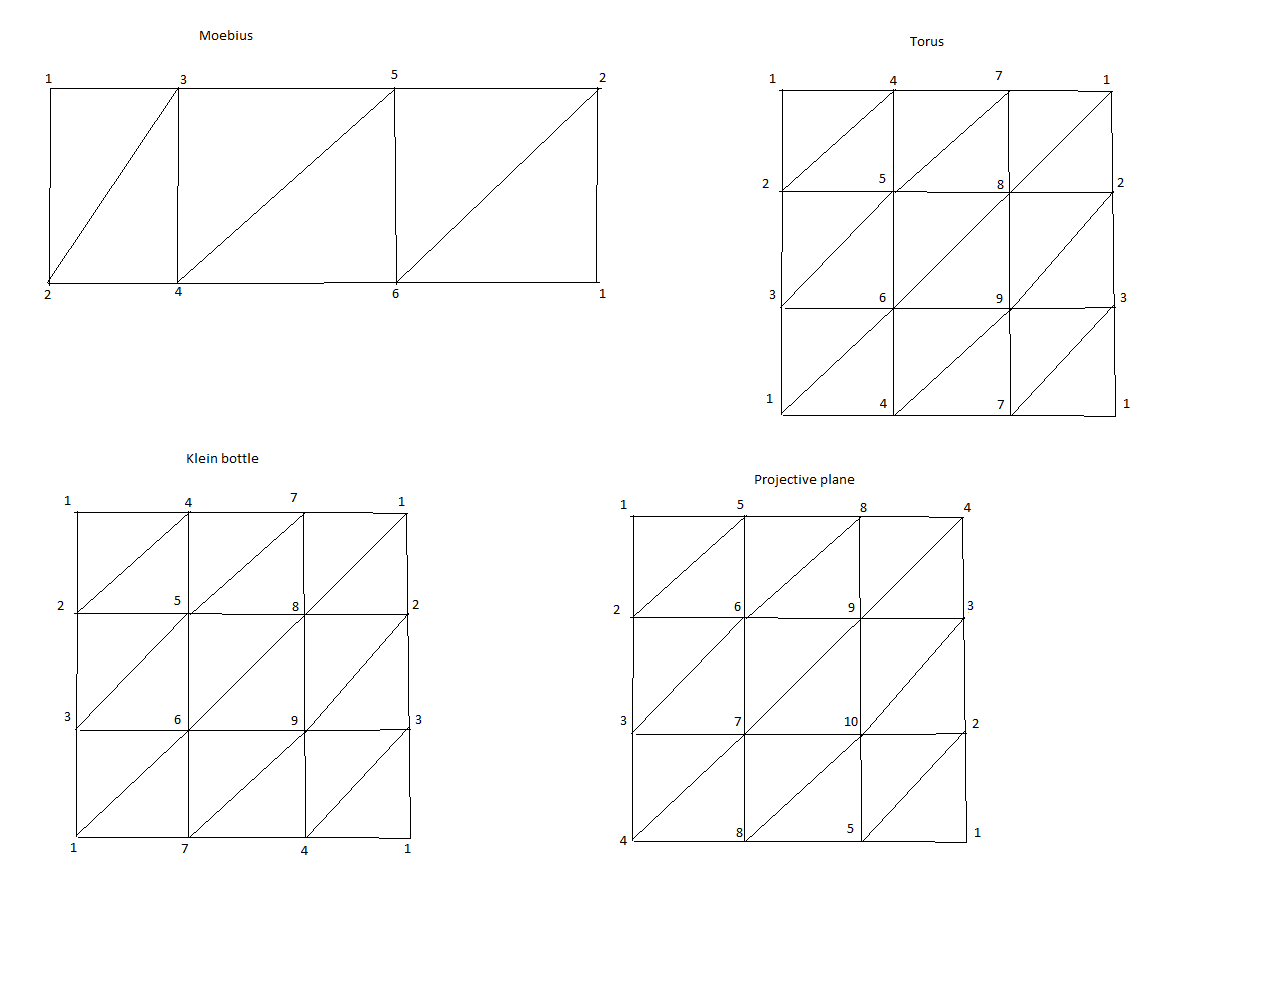
\includegraphics[width=400px]{filtrations.png}

Pour chacune, nous avons pris la convention de mettre la valeur 
égale à la dimension, ce qui assure la consistance de la filtration. 
Les fichiers \texttt{.txt} sont disponibles dans le dossier 
\texttt{data}. Pour les sphères et les boules, celles-ci ont été 
générées grâce au scipt \texttt{ballgen.py} également présent dans
ce dossier.

\vskip 0.5cm

On retrouve les nombres attendus pour les exemples connus que sont 
les sphères, les boules et le tore.On peut voir ci-dessous les
résultats pour la bande de Moebius, la bouteille de Klein et le
plan projectif.

\pagebreak

\begin{figure}[h!]
    \caption{Ruban de Moebius}
    \centering
    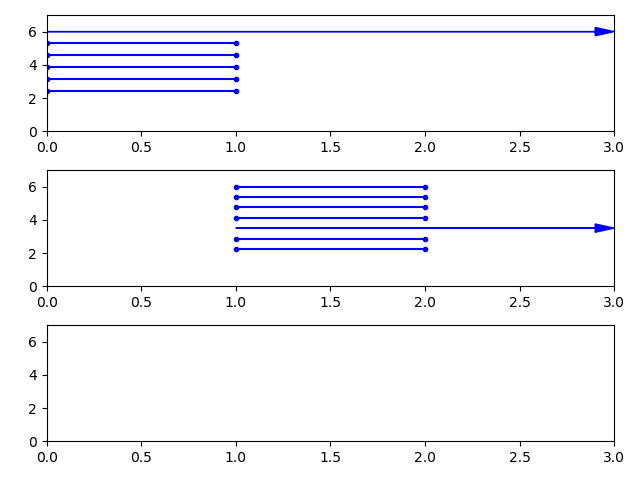
\includegraphics[height=150px]{moebius.png}
\end{figure}

\begin{figure}[h!]
    \caption{Bouteille de Klein}
    \centering
    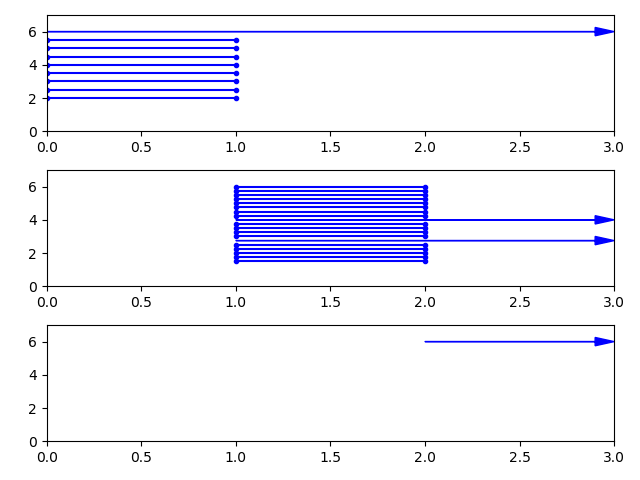
\includegraphics[height=150px]{klein.png}
\end{figure}

\begin{figure}[h!]
    \caption{Plan projectif}
    \centering
    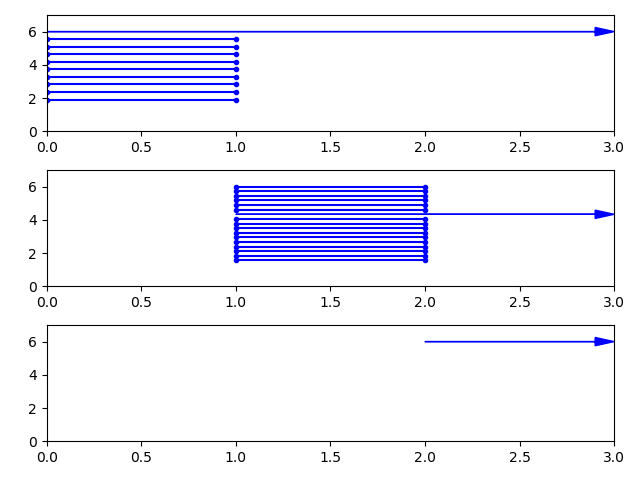
\includegraphics[height=150px]{projective.png}
\end{figure}



\pagebreak


\section{Analyse sur les données fournies}

\subsection{Performance}

\begin{itemize}
    \item[\textbf{filtration A}] \hspace{1cm}
        \begin{itemize}
            \item[Création de la matrice :] 43 secondes % (13 minutes 21 secondes sans la table de hachage)
            \item[Réduction de la matrice :] 18 minutes 55 secondes 
        \end{itemize}
    \item[\textbf{filtration B}] \hspace{1cm}
        \begin{itemize}
            \item[Création de la matrice :] 10 secondes % (51 secondes sans la table de hachage)
            \item[Réduction de la matrice :] 50 secondes 
        \end{itemize}
    \item[\textbf{filtration C}] \hspace{1cm}
        \begin{itemize}
            \item[Création de la matrice :] 20 secondes % (2 minutes 3 secondes sans la table de hachage)
            \item[Réduction de la matrice :] 2 minutes 3 secondes 
        \end{itemize}
    \item[\textbf{filtration D}] \hspace{1cm}
        \begin{itemize}
            \item[Création de la matrice :] 4 minutes 32 secondes
            \item[Réduction de la matrice :] 1 heure 42 minutes 47 secondes
            (la réduction s'est bloquée longtemps à 96\% des colonnes
            réduites, étape atteinte en 3 minutes et 30 secondes)  
        \end{itemize}
\end{itemize}

\subsection{Analyse}

\begin{itemize}
    \item[\textbf{filtration A}]
        On peut imaginer que la structure originelle est celle 
        d’une sphère. Il faut un certain temps pour que tous les 
        points fusionnent ensemble, d’où l’apparition de nombreuses 
        composantes connexes et de petits cycles. Une fois tous les 
        points liés et les faces apparues, on peut observer la 
        structure de sphère par la large barre sur H2. Enfin, la 
        boule finit par se remplir, d’où la fin de la barre.
    \item[\textbf{filtration B}]
        On voit plusieurs phénomènes : d’abord 8 trous d’ordre 2 
        faisant penser à 8 petites sphères, puis l’apparition de 5 
        trous de dimension 1 et enfin, au moment où ils disparaissent, 
        l’apparition d’un trou de dimension 2. Cela fait penser à la 
        structure que l’on obtiendrait en disposant 8 sphères dont les 
        centres seraient les sommets d’un cube et qui auraient chacune 
        un point en commun avec chacune de ses voisines. Il y aurait 
        donc un trou par face, mais le sixième est linéairement 
        dépendant des 5 autres, d’où l’apparition de 5 barres. Au 
        moment où ces 5 cycles disparaissent, cela signifie que les 
        faces sont maintenant pleines. Mais au centre du cube, un 
        espace n’est pas encore atteint, d’où l’apparition d’un trou 
        d’ordre 2. La forme sous-jacente est donc celle de 8 sphères 
        placées au sommet d’un cube  de côté égal au diamètre des 
        sphères (le cube ne sert qu’à se représenter la disposition, 
        il n’est pas réellement tracé).
    \item[\textbf{filtration C et D}]
        Les filtrations C et D ont toutes les deux des diagrammes 
        similaires, avec deux principaux trous d’ordre 1 et d’ordre 2. 
        On reconnait là la structure d’un tore. De plus, le fait qu’un 
        trou disparait en même temps que le vide de dimension 2 
        correspond au moment où le tore devient plein pour prendre une 
        structure “d’anneau plein” (de cercle). La différence entre 
        les deux provient du fait que le C est beaucoup plus fin que le D.
\end{itemize}


\end{document}